\chapter{Results}
\label{cha:results}


This chapter discusses the basic findings of the analysis of the proposed peer influence model.
All results were obtained from synthetic networks that were generated over \( T = 75,000 \) iterations.
The size of the networks was fixed to \(n = 5,000 \) nodes and since the model heavily depends on events that happen at random are the reported properties of the time-varying networks obtained by averaging the results of 40 independent runs.
The model parameter that are responsible for the formation of the community structures are set to \( p_{\Delta} = 0.90 \) for the triadic closure probability, \( \delta = 1 \) for the link reinforcement constant, and \( p_{d} = \num{5e-05} \) for the node deletion probability for every experiment.
Furthermore, the critical peer influence threshold was fixed to \( \theta = 0.10 \).
This reflects the idea that only a relatively small number of active neighbors is sufficient to increase the activity of a node in a significant way.

The topological properties of the integrated network, which are discussed in \cref{sec:integrated-network-properties}, are measured only for nodes that are part of the temporal network.
This means that nodes that were removed earlier due to the node deletion process do not influence the properties of the integrated network any more.
\Cref{sec:network-activity} contains an overview of the overall network activity with respect to different levels of peer influence.
The effect of the peer influence mechanism on the inter-event time distribution in the network is examined in \cref{sec:inter-event-time-dists}.
All this experiments are performed for different values for the maximum peer influence probability \( q \).
However, the last section (\cref{sec:softmax-rescaling}) keeps the peer influence level constant and discusses how different values for \( \beta \), the inverse temperature for the softmax weight re-scaling, change the peer influence effects in the network.
The synthetic networks that are used in the first three sections use the average tie strength as temperature for the softmax weight re-scaling.
Therefore, \( \beta \) is set to the to the inverse of the average of the weights in the integrated network in each iteration after the first one.
The value is set to \( \beta = 1 \) in the initial round to avoid division by zero, due to the fact that the network is completely disconnected in the beginning.


%% ========================================================================
%% ========================================================================


\section{Integrated Network Properties}
\label{sec:integrated-network-properties}

Not only the integrated network of all 75,000 previous instantaneous networks and its properties are of great interest, but also how they evolve during the simulation.
This allows to get a deeper understanding on how the model shapes the community structures in the network.
To make this possible is the integrated network build in an iterative fashion.
A snapshot of it is taken after the newly formed ties are added and the weights of already established links are updated in every time step.
Features like the average local clustering coefficient or the average weight of the ties are then calculated for everyone of the 75,000 integrated network snapshots.
This allows to examine on how the topology and other measures change over time.

The first, and most interesting, measure that can be investigated in this way is the average local clustering coefficient \( C(t) \).
\Cref{fig:avg-local-cc-full} depicts the development of it over the course of the simulation for different levels of peer influence.


\myfig{avg-local-cc-full}
      {width=0.75\textwidth}
      {Foo}
      {Evolution of the average local clustering coefficient}
      {fig:avg-local-cc-full}

\begin{figure}[htbp]
  \centering
  \begin{subfigure}[b]{0.48\textwidth}
    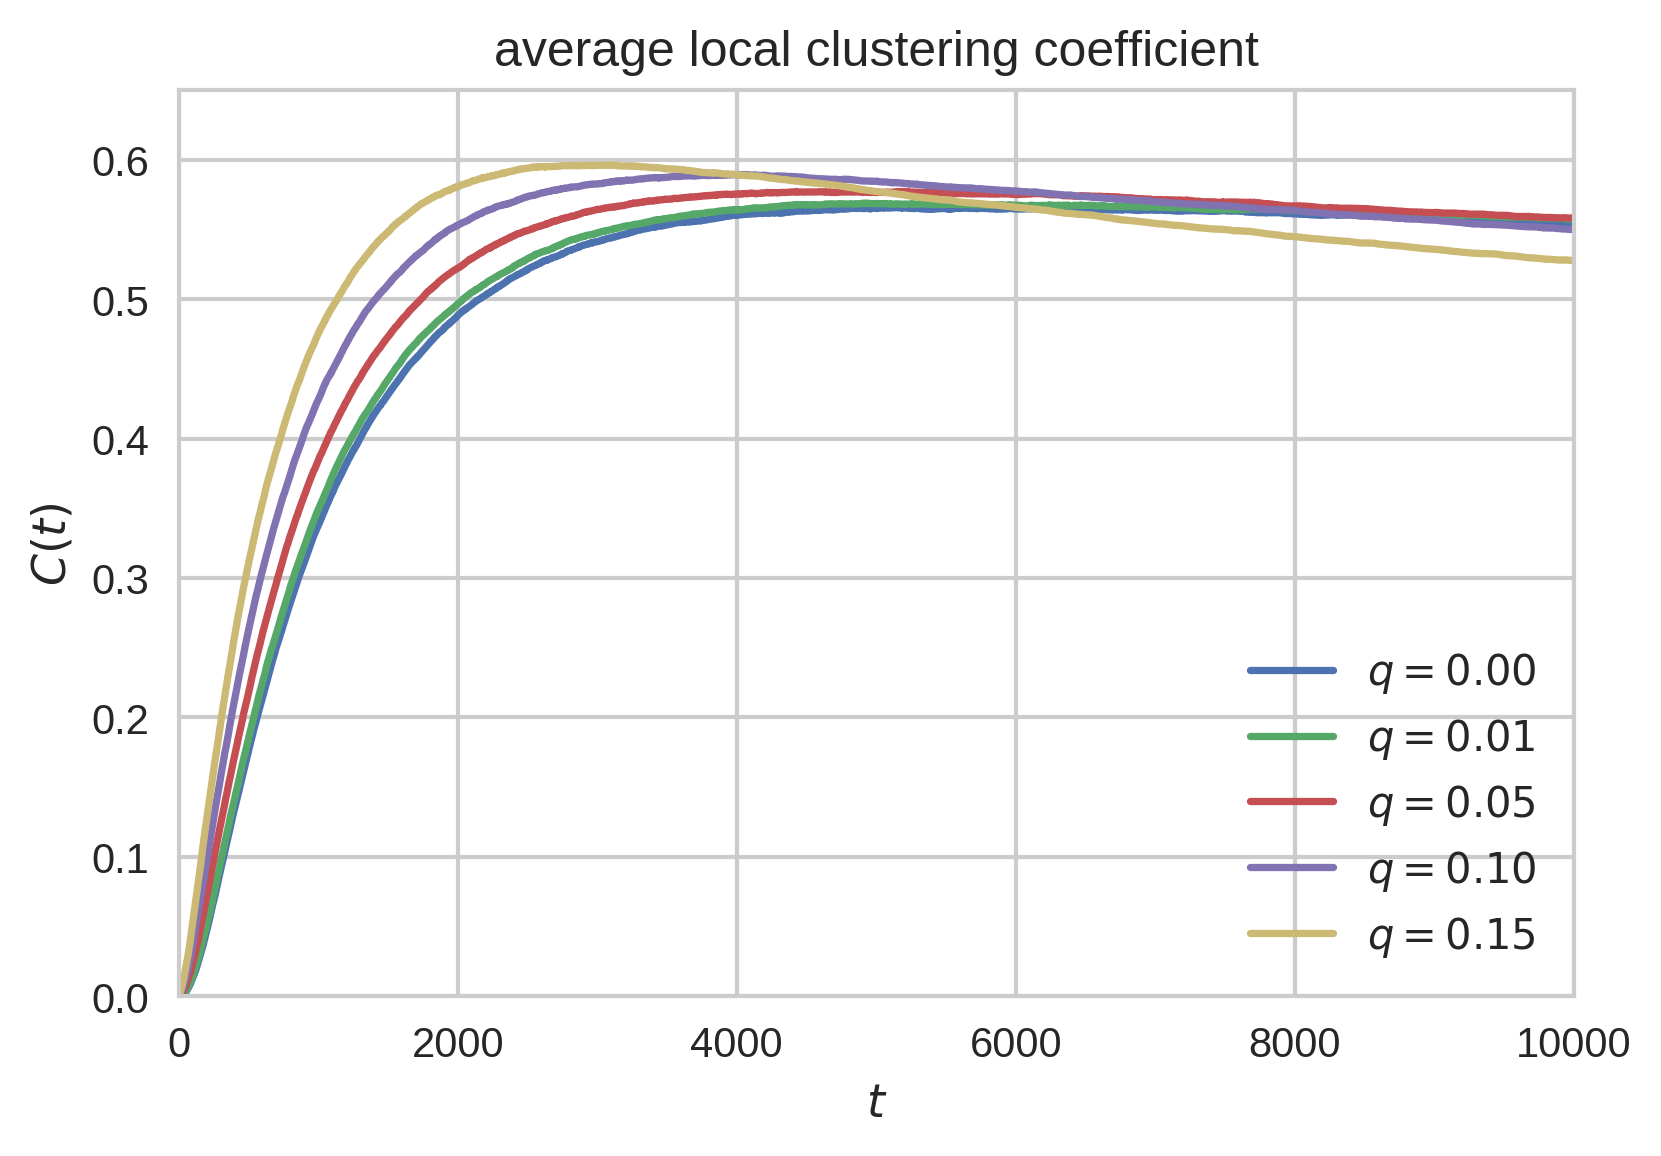
\includegraphics[width=\textwidth]{figures/avg-local-cc-start}
    \caption{}
    \label{subfig:avg-local-cc-start}
  \end{subfigure}
  ~
  \begin{subfigure}[b]{0.48\textwidth}
    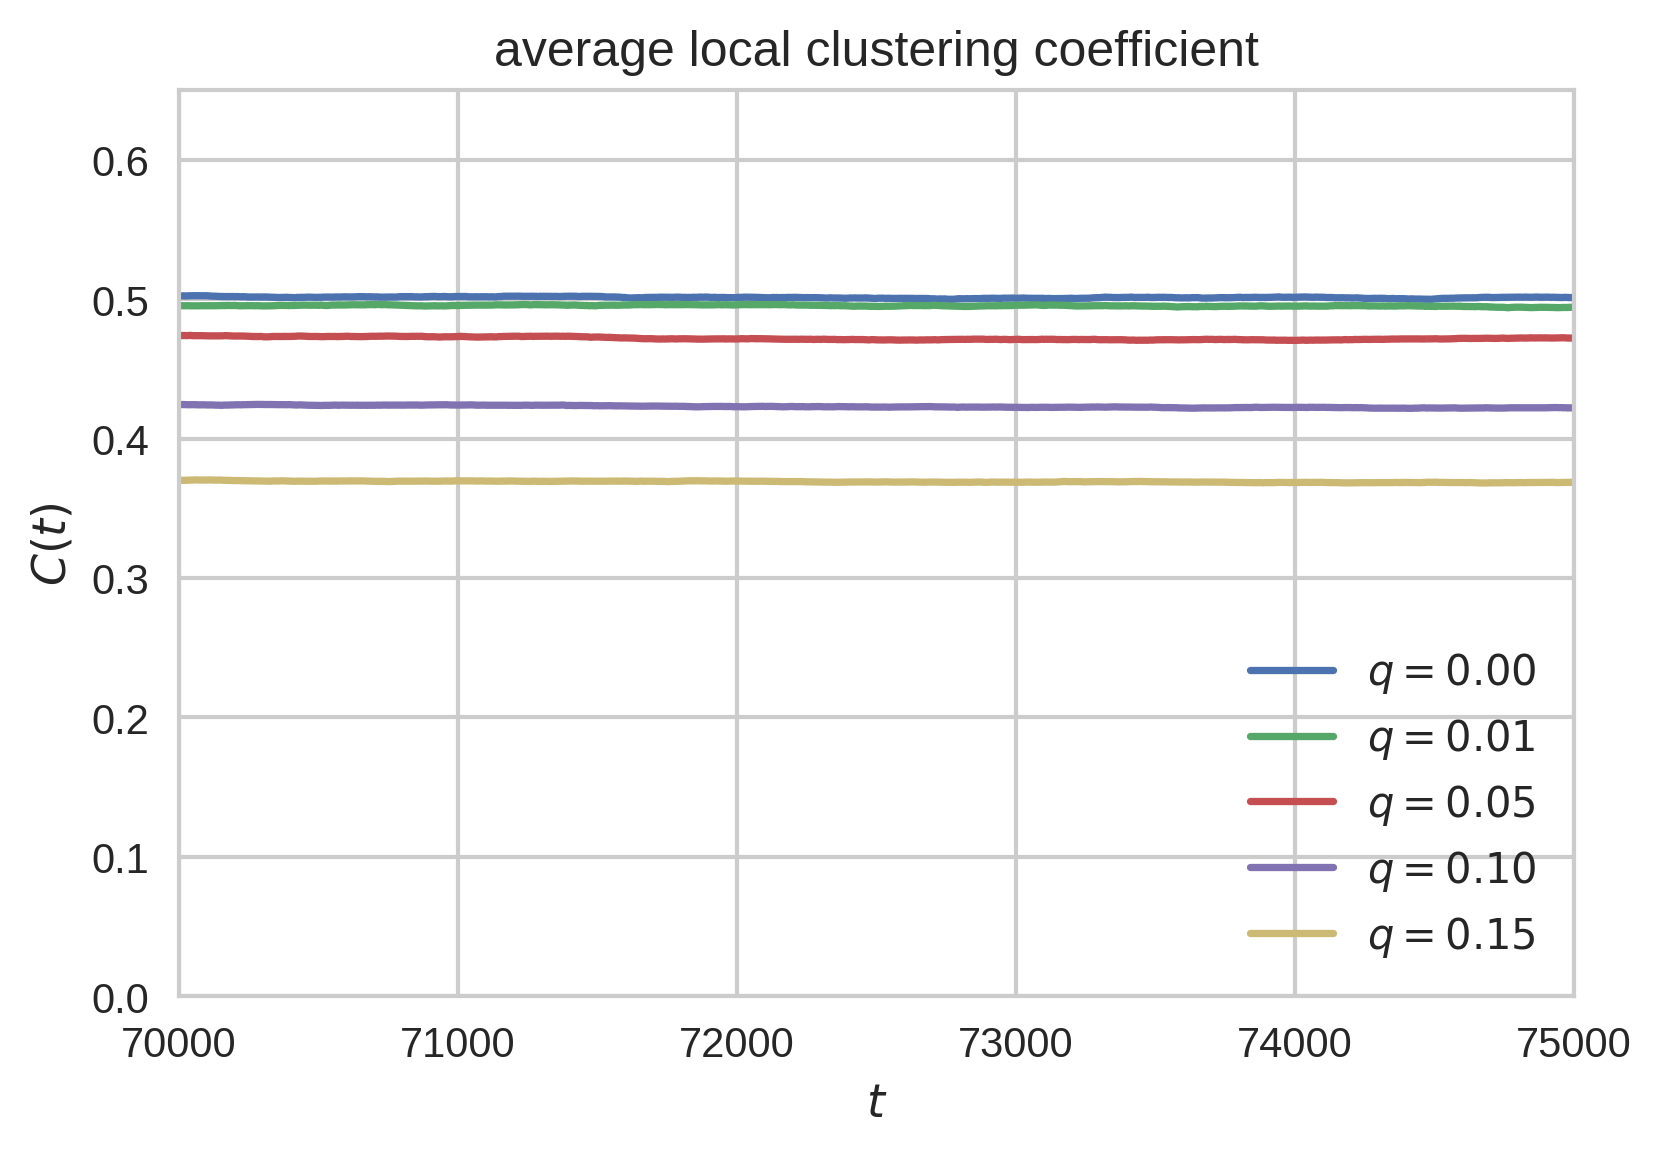
\includegraphics[width=\textwidth]{figures/avg-local-cc-end}
    \caption{}
    \label{subfig:avg-local-cc-end}
  \end{subfigure}

  \caption[details]{details}
  \label{fig:avg-local-cc-start-and-end}
\end{figure}


%% ========================================================================
%% ========================================================================


\section{Network Activity}
\label{sec:network-activity}


%% ========================================================================
%% ========================================================================


\section{Inter-event Time Distributions}
\label{sec:inter-event-time-dists}
% definition burstiness and parameter B is invariant wrt to activity homogeneity in \cite{Goh2008}
% nice explanation for B in \cite{Masuda2016}


%% ========================================================================
%% ========================================================================


\section{Softmax Weight Re-scaling}
\label{sec:softmax-rescaling}
